% Methodology -- handbook section 3

\subsection{Pipeline overview}
\label{subsec:methodology-1}
% Required: Diagram of the form: raw data, preprocessing, dataloader, model, loss, optimization, prediction, post-processing, evaluation.

Figure~\ref{fig:pipeline} shows the path from the raw archives to a reported number. Every
configuration in this report takes the identical path; only the blocks named in
Section~\ref{subsec:methodology-4} change, one at a time, which is what makes a difference in
score attributable to the factor varied rather than to the pipeline around it.

\begin{figure}[H]
    \centering
    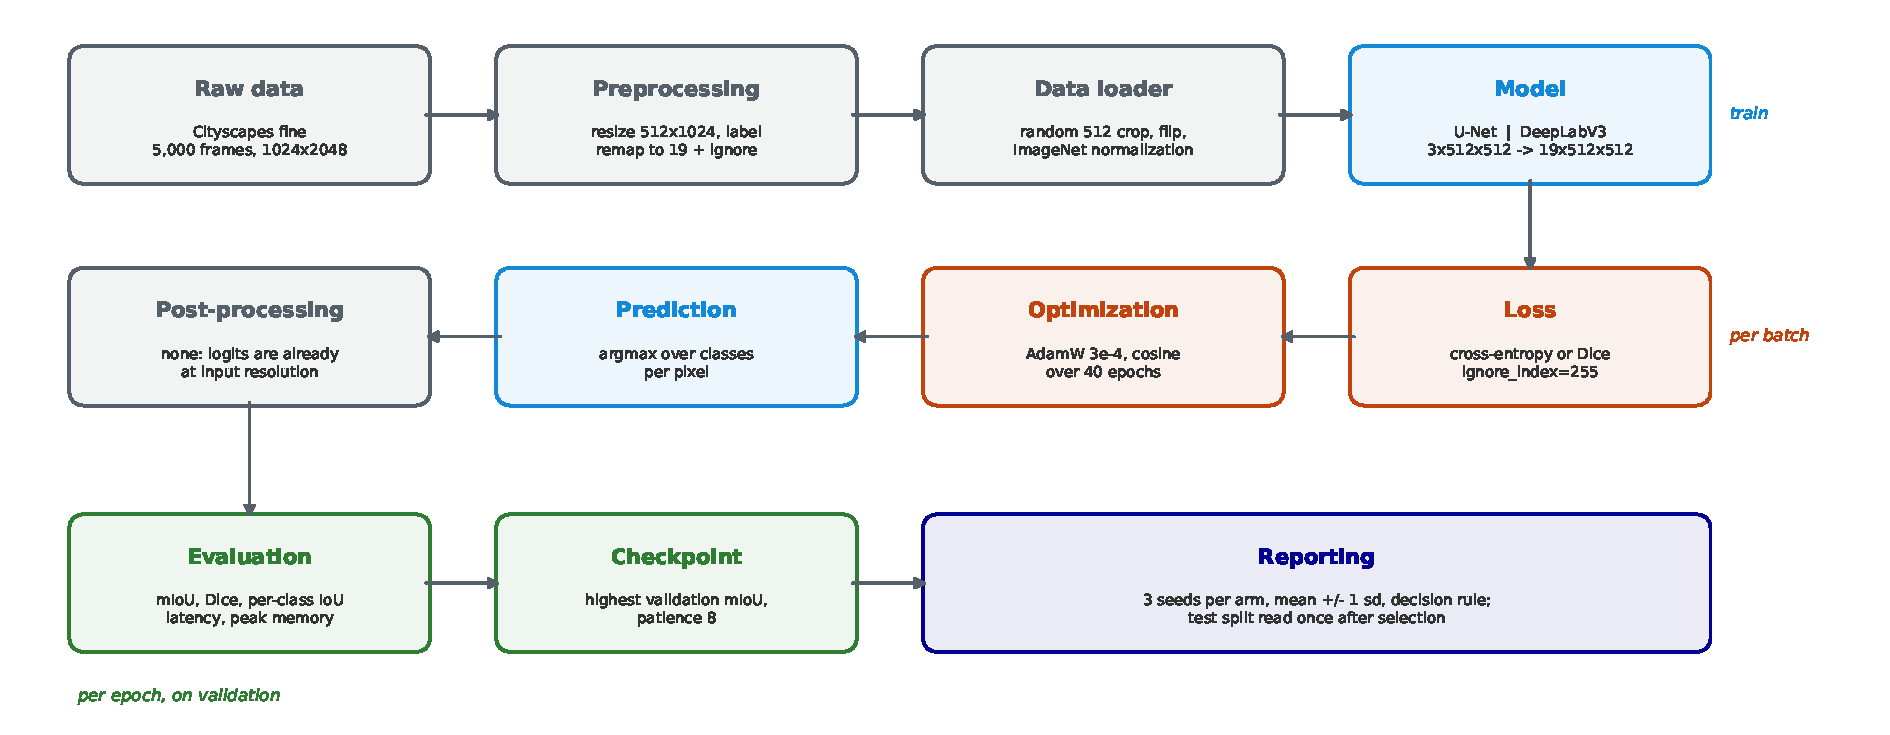
\includegraphics[width=\textwidth]{images/pipeline.pdf}
    \caption{The pipeline.}
    \label{fig:pipeline}
\end{figure}

Two stages deserve a note. Post-processing is empty by design: both models emit logits at the
input resolution, so the prediction is an \texttt{argmax} and nothing is upsampled, smoothed or
thresholded afterwards. And evaluation runs twice on different terms. Validation is computed
every epoch and selects the checkpoint; the test split is read once per configuration, after
selection has concluded.

\subsection{Baseline and main methods}
\label{subsec:methodology-2}
% Required: Architecture, input representation, loss, metrics, strengths and limits, parameter count. State which parts were self-implemented and which came from libraries, naming the libraries.
% Also required: Section 20: a simple baseline, at least one pretrained or modern model, and a clear fine-tuning procedure.

Both models consume the identical input representation, a $3 \times 512 \times 512$ crop
normalised as Section~\ref{subsec:problem-and-data-5} describes, and emit
$19 \times 512 \times 512$ logits scored by the same metrics. They differ in where their features
come from: one learns everything from $2{,}406$ frames, the other starts from weights fitted on a
far larger corpus.

\textbf{U-Net, the baseline.} A symmetric encoder and decoder \cite{ronneberger2015unet} written
from scratch, base width $32$ and depth $4$, with no pretrained weights. Each encoder stage
applies two padded $3 \times 3$ convolutions, each batch-normalised and rectified, then halves
the resolution by max pooling; widths double at every level, $32 \to 64 \to 128 \to 256$, and a
$512$-wide block bridges the bottom. The decoder mirrors this, upsampling by transposed
convolution and ending in a $1 \times 1$ convolution to the 19 logits. Formally, writing $e_\ell$
for the encoder map at level $\ell$ and $d_\ell$ for its decoder counterpart,

\begin{equation}
    e_\ell = \mathrm{DoubleConv}(\mathrm{MaxPool}_2(e_{\ell-1})), \qquad
    d_\ell = \mathrm{DoubleConv}([\,\mathrm{ConvT}_2(d_{\ell+1});\, e_\ell\,]),
    \label{eq:unet}
\end{equation}

where $[\cdot\,;\cdot]$ concatenates along channels. The skip connection in
Equation~\ref{eq:unet} is the point of the architecture rather than a detail of it: four
poolings reduce a $512$-pixel crop to $32$ pixels, which carries enough context to say what a
region is but is far too coarse to say where its boundary runs, so each decoder stage places the
upsampled semantics back onto the encoder detail that produced them. Padding keeps every
convolution at its input size, so a skip always meets a map of exactly matching resolution.
Convolutions carry no bias because each is followed by batch normalisation, which recentres the
activations and makes the bias redundant. The model holds $7{,}763{,}635$ parameters, all
trainable. Its strength is that it is fully determined by this data; its limit is that it must
learn every edge and texture detector from $2{,}406$ frames.

\textbf{DeepLabV3, the pretrained model.} Torchvision's DeepLabV3 \cite{chen2017deeplabv3} with a
MobileNetV3-Large backbone \cite{howard2019mobilenetv3}, pretrained on a COCO subset
\cite{lin2014coco} carrying the twenty VOC classes, over an ImageNet-pretrained
\cite{deng2009imagenet} classification backbone. It replaces the U-Net's decoder with atrous
convolution: the backbone's final stages use dilated kernels so the feature map is never reduced
below a stride of $8$, and an atrous spatial pyramid pooling module gathers context at several
dilation rates in parallel before a $1 \times 1$ convolution produces the logits, which a single
bilinear interpolation returns to the input resolution. The published head predicts 21 classes,
so its final $1 \times 1$ convolution is replaced by a 19-class one; the backbone and the pooling
module transfer unchanged, since they carry the learned features. The model holds $11{,}024{,}963$ parameters.

Two implementation details matter for the comparison. The auxiliary head the architecture can
carry is removed rather than computed and discarded, so training pays nothing for an output no
loss reads. And the normalization is taken from the weights' own transform rather than assumed,
for the reason given in Section~\ref{subsec:problem-and-data-5}.

\textbf{Fine-tuning procedure.} A single stage, with no schedule of its own. The final
convolution is replaced for the 19 classes, and every parameter trains from the first epoch at
one learning rate: no layer is unfrozen part way through and no layer carries a separate rate.
This is deliberate, because it is the procedure the U-Net also receives, so
Section~\ref{subsec:results-4} compares models rather than training schedules. The controlled
experiment varies exactly this choice by freezing the backbone, which leaves $8{,}053{,}011$ of the $11{,}024{,}963$ parameters trainable. That the
frozen arm still trains $73\%$ of the model is not a mistake but a property of the architecture:
the pooling module and classifier hold $8.05$M parameters against the backbone's $2.97$M, so
freezing a MobileNetV3 backbone removes far less than the word suggests.
Section~\ref{subsec:results-4} returns to this.

\textbf{Backbone variant.} The extension replaces MobileNetV3-Large with ResNet50
\cite{he2016resnet}, giving $39{,}638{,}355$ parameters, $3.6$ times the baseline backbone, under
an otherwise identical procedure.

\textbf{Losses and metrics.} The default objective is the pixel cross-entropy of
Equation~\ref{eq:cross-entropy}. The ablation replaces it with a soft Dice loss
\cite{milletari2016vnet} computed over the same labelled pixels $\Omega$,

\begin{equation}
    \mathcal{L}_{\mathrm{Dice}}(\theta) = 1 - \frac{1}{C} \sum_{c=1}^{C}
    \frac{2 \sum_{(i,j) \in \Omega} p_{cij}\, \mathbf{1}[y_{ij} = c] + \varepsilon}
         {\sum_{(i,j) \in \Omega} p_{cij} + \sum_{(i,j) \in \Omega} \mathbf{1}[y_{ij} = c] + \varepsilon},
    \qquad \varepsilon = 1,
    \label{eq:dice}
\end{equation}

with $p = \mathrm{softmax}(z)$. The two differ in what they weight. Cross-entropy averages over
pixels, so a class contributes in proportion to the ground it covers; Dice averages over classes,
so a pole counts as much as the road. Equation~\ref{eq:dice} averages over all $C$ classes
whether or not the batch contains them, a property Section~\ref{subsec:results-6} shows to be
consequential.

Mean intersection over union is the primary metric, with Dice, per-class IoU and pixel accuracy
secondary. Both are computed from one running $19 \times 19$ confusion matrix accumulated over a
split, never from concatenated masks, since a validation pass at $512 \times 1024$ holds
$298$ million pixels. For class $c$ with true positives $\mathrm{TP}_c$, false positives
$\mathrm{FP}_c$ and false negatives $\mathrm{FN}_c$,

\begin{equation}
    \mathrm{IoU}_c = \frac{\mathrm{TP}_c}{\mathrm{TP}_c + \mathrm{FP}_c + \mathrm{FN}_c},
    \qquad
    \mathrm{Dice}_c = \frac{2\,\mathrm{TP}_c}{2\,\mathrm{TP}_c + \mathrm{FP}_c + \mathrm{FN}_c},
\end{equation}

and mIoU is the mean over the classes present in the split: a class absent from the ground truth
is excluded from the average rather than scored zero. Pixel accuracy is
recorded but never decides a comparison, for the reason measured in
Section~\ref{subsec:problem-and-data-3}.

\textbf{Implementation.} The U-Net, the Dice loss, the confusion matrix and every metric derived
from it, the training loop, the evaluation, the experiment runner and the figures are written by
the group. DeepLabV3 and its pretrained weights come from torchvision; layer primitives
(\texttt{nn.Conv2d}, \texttt{nn.ConvTranspose2d}, \texttt{nn.BatchNorm2d},
\texttt{nn.MaxPool2d}), cross-entropy, AdamW and the cosine schedule come from PyTorch
\cite{paszke2019pytorch}; the label-id table is read from \texttt{cityscapesscripts}; the plots
come from matplotlib.

\subsection{Training setup}
\label{subsec:methodology-3}
% Required: Optimizer; learning rate; batch size; epochs; scheduler; regularization; early stopping; checkpoint criterion; seed; hardware; mixed precision if used; training time; hyperparameter selection method.

Every configuration is trained under the identical protocol of Table~\ref{tab:protocol}. A run
that deviates from it is repeated rather than reported.

\begin{table}[H]
\centering
\caption{Shared training protocol.}
\label{tab:protocol}
\begin{tabularx}{\textwidth}{lX}
\hline
\textbf{Setting} & \textbf{Value} \\
\hline
Input                & Resized to $512 \times 1024$; training takes a random $512 \times 512$ crop, evaluation the whole resized frame \\
Optimizer            & AdamW \cite{loshchilov2019adamw}, $\eta = 3 \times 10^{-4}$, weight decay $\lambda = 0.05$, over the parameters that require gradients \\
Batch size           & 8, giving 301 steps per epoch \\
Epochs               & 40 maximum \\
Scheduler            & Cosine annealing, stepped once per epoch, period equal to the 40 configured epochs \\
Regularization       & Weight decay; random crop and horizontal flip on the training loader only; no dropout \\
Early stopping       & After 8 epochs without an improvement in validation mIoU \\
Checkpoint criterion & Highest validation mIoU \\
Seeds                & $0$, $1$ and $2$ for every configuration entering a comparison \\
Hardware             & Apple M4 Pro, 14 cores, 48~GB unified memory, MPS backend \\
Software             & Python 3.12.0, PyTorch 2.14.0, torchvision 0.29.0 \\
Mixed precision      & Not used; all runs are full \texttt{float32} \\
Training time        & 25.5 hours over 13 runs, from 0.50~h to 8.22~h per run \\
\hline
\end{tabularx}
\end{table}

\textbf{Hyperparameter selection.} None was performed. The optimizer, schedule and budget were
fixed in advance from values conventional for AdamW on a dense prediction task and applied
unchanged to every arm, since tuning them per arm would confound the comparison with unequal
search effort. Each configuration ran once, at a setting fixed
before training, and an experiment changes exactly one of those settings. The search effort is
therefore zero and identical across arms, and every score in this report is
a score under a common protocol at an untuned configuration rather than the best that
configuration could reach.

Early stopping interacts with the schedule in one way worth stating: it does not shorten the
cosine period, so a run that stops early ends above the minimum learning rate rather than at it.

\textbf{Reproducibility, and its limit on this hardware.} Each seed sets the Python, NumPy and
PyTorch generators together, and every run records the configuration it resolved to, the software
versions it ran under and the commit it was produced at. One limit is imposed by the hardware and
is reported rather than hidden. Deterministic algorithms are requested, but the Apple GPU backend
provides no deterministic kernel for the scatter-add that DeepLabV3 reaches in the backward pass
of the bilinear interpolation returning its logits to full resolution, so PyTorch warns and
proceeds nondeterministically rather than failing.
Measured at a fixed seed, the U-Net reproduces bit-exactly while DeepLabV3 diverges by about
$4 \times 10^{-7}$ per step. The seed-to-seed spread reported throughout
Section~\ref{sec:results} consequently includes this nondeterminism for the DeepLabV3 arms, and
rerunning one of those seeds will not reproduce its number exactly.

\subsection{Experimental design}
\label{subsec:methodology-4}
% Required: Per experiment: hypothesis; changed factor; fixed factors; metrics; conclusion criteria.
% Also required: Section 20: at least one controlled experiment, such as freeze versus full fine-tune, with versus without augmentation, backbone A versus B, loss A versus B, or resolution A versus B.

Four experiments are reported. Each was stated in full, with its hypothesis and its decision
criterion, before the runs were launched. Table~\ref{tab:experiments} summarises them: each
changes one thing and holds the rest of Table~\ref{tab:protocol} fixed.

\begin{table}[H]
\centering
\caption{The experiment matrix.}
\label{tab:experiments}
\small
\begin{tabularx}{\textwidth}{lXr}
\hline
\textbf{Role} & \textbf{Factor varied} & \textbf{Seeds} \\
\hline
Model comparison       & U-Net trained from scratch against the pretrained DeepLabV3 & $3 + 3$ \\
Controlled experiment  & Backbone frozen against fully fine-tuned & $3$ \\
Ablation               & Cross-entropy against Dice loss & $3$ \\
Backbone extension     & MobileNetV3-Large against ResNet50 & $1$ \\
\hline
\end{tabularx}
\end{table}

\textbf{The model comparison.} \emph{Hypothesis:} the pretrained DeepLabV3 outperforms the U-Net
trained from scratch at comparable capacity, $11.0$M against $7.8$M parameters, because
$2{,}406$ training images are too few to learn general features from scratch. \emph{Varies:} the
model. \emph{Fixed:} the split, the protocol, the loss, the normalization and the seed set.
\emph{Metrics:} mIoU primary; Dice, per-class IoU, parameter count, seconds per epoch and
inference latency secondary.

\textbf{The controlled experiment: frozen against fully fine-tuned backbone.}
\emph{Hypothesis:} fine-tuning every parameter outperforms training the head on a frozen
backbone, because features fitted to object-centric photographs are not adapted to street scenes;
the gap is widest on thin classes such as pole and traffic sign, whose boundaries depend on
low-level features the frozen arm cannot change. \emph{Varies:} whether the backbone receives
gradients. \emph{Fixed:} backbone, pretrained weights, head, learning rate and the rest of the
protocol. \emph{Metrics:} mIoU and per-class IoU, trainable parameters, seconds per epoch. One
consequence of freezing is stated in advance: the backbone stops learning but stays in training
mode, so its batch-normalization running statistics still adapt to Cityscapes. The frozen arm
fixes every learned weight but not those statistics.

\textbf{The ablation: cross-entropy against Dice loss.} \emph{Hypothesis:} Dice raises IoU on
classes that are rare but large when present, namely train, bus and truck, because it weights
every class equally regardless of pixel count; it does not help thin classes, whose errors lie at
boundaries rather than in how often the class is seen. \emph{Varies:} the training objective.
\emph{Fixed:} the fully fine-tuned DeepLabV3-MobileNetV3 and the protocol. \emph{Metrics:} mIoU
and Dice, and per-class IoU for train, bus, truck, pole and traffic sign. The hypothesis holds
only if the per-class rule separates the two arms on at least two of train, bus and truck.

\textbf{The backbone extension.} \emph{Hypothesis:} ResNet50 outperforms MobileNetV3-Large at
$3.6$ times the parameters and roughly $7$ times the cost per step. \emph{Varies:} the backbone.
\emph{Fixed:} full fine-tuning, cross-entropy and the protocol. \emph{Metrics:} mIoU, parameter
count, seconds per epoch, inference latency. Run at seed $0$ only, so it is reported as
indicative and cannot substitute for the controlled experiment or the ablation.

\textbf{Conclusion criterion.} Fixed before any result was seen and applied to every comparison
in this report. Configuration $A$ is reported as better than $B$ only when the mean validation
mIoU of $A$ exceeds that of $B$ \emph{and} the two intervals of mean $\pm$ one standard deviation
across the three seeds do not overlap. Overlapping intervals mean the two are indistinguishable
under this protocol, which is itself a result and is not resolved by picking the higher mean. A
claim about a single class applies the same rule to that class's IoU. A configuration run at one
seed supports no claim of superiority.
